\chapter{Grundlagen}
\label{sec:FUNDAMENTALS}

In diesem Kapitel werden die Grundlagen für diese Arbeit vorgestellt. Zu diesen Grundlagen gehört zu erst einmal die eingesetzten Technologien.

\section{Containervirtualisierung}
\label{sec:FUNDAMENTALS_CONTAINER}

In der Informatik bezeichnet der Begriff Virtualisierung ein Framework zur Trennung der Ressourcen eines Computers in mehrere Ausführungsumgebungen \cite{virtualization}. Dies kann durch Konzepte oder Technologien wie Hard- oder Software-Partitionierung, Time-Sharing, teilweise oder gänzliche Maschinen Simulation oder auch Emulation realisiert werden. Dabei existieren verschiedene Arten der Virtualisierung. Bei der Hardwarevirtualisierung oder Emulation geht es um den Computers als gesamte Hardware Plattform \cite{wiki:hardware_virtual}. Dadurch ist es möglich parallel neben einem fest installiertem Betriebssystem, auch Hostsystem genannt, auf einem Computer weitere simulierte Computerumgebungen mit einem Betriebssysteme als Gastsysteme auszuführen. Diese werden allgemein auch als \ac{vm} bezeichnet. Dabei besteht keine Einschränkung hinsichtlich des genutzten Betriebssystems als Gastsystem. Somit ist es möglich z.B. auf einem Hostsystem mit Windows ein Gastsystem mit einem Linux basiertem Betriebssystem zu betreiben. Der umgekehrte Fall ist entsprechend auch möglich. Des Weiteren sind aufgrund der Abstraktionsschicht durch die Virtualisierung die einzelnen \acp{vm} vom Hostsystem und anderen Gastsystemen isoliert und ein Zugriff auf diese wird unterbunden. Die vollständige Isolierung konnte jedoch selbst in der jüngsten Vergangenheit nicht immer zu 100\% sichergestellt werden \cite{CVE-2017-4934}.

Eine weitere Art der Virtualisierung wird als Software- oder auch Containervirtualisierung bezeichnet \cite{software_container}. Historisch hat sich die Containervirtualisierung aus der Unix-System Operation chroot entwickelt. Chroot ermöglicht die Zugriffe eines Prozesses auf ein Unterverzeichnis zu limitieren. Aus den Konzepten der chroot-Operation haben sich die heutigen \ac{lxc} entwickelt. \ac{lxc} bauen auf Standard Funktionalitäten des Linux Kernels auf und isolieren anhand von Kernel Namespaces und cgroups die Ausführung eines Programms. Kernel Namespaces isolieren dabei mit eigenen Prozess-IDs, Dateisystem, Netzwerk und Benutzer-IDs ein Programm vom Hostsystem. Wiederrum limitieren und priorisieren cgroups die Ressourcen eines Computers wie z.B. CPU, Arbeitsspeicher oder Netzwerk. Anders als bei einer \ac{vm} wird nicht ein ganzes Betriebssystem in einer virtualisierten Umgebung ausgeführt, sondern, wie in Abbildung~\ref{fig:DOCKER_VS_VM} auf Seite~\pageref{fig:DOCKER_VS_VM} zusehen, nur einzelne Programme. Dabei kann ein Programm aus einem Hauptprozess und mehreren Subprozessen bestehen. Die virtuelle Umgebung eines einzelnen Programms wird als Container bezeichnet. Container haben in vielen Szenarien signifikante Geschwindigkeitsvorteile gegenüber \acp{vm} \cite{performance_container}. Neben den Ressourcen eines Computers nutzen alle Container denselben Betriebssystem Kernel. Jedoch können verschiede Linux Distributionen unabhängig vom Hostsystem innerhalb der Container zur Verfügung gestellt werden. Somit findet die Virtualisierung der Container auf der Ebene des Betriebssystem statt und ist im Fall von \ac{lxc} von bestimmten Funktionalitäten des Linux Kernels abhängig. Dank \ac{lxc} ist die Containervirtualisierung auf allen Linux basierte Distribution möglich, aber es ist auch genau auf diese limitiert und die Portabilität auf andere Kernel bedingt die Unterstützung einer ähnlicher Funktionalität zur Virtualisierung auf Ebene des Betriebssystems.

\begin{figure}
    \centering
    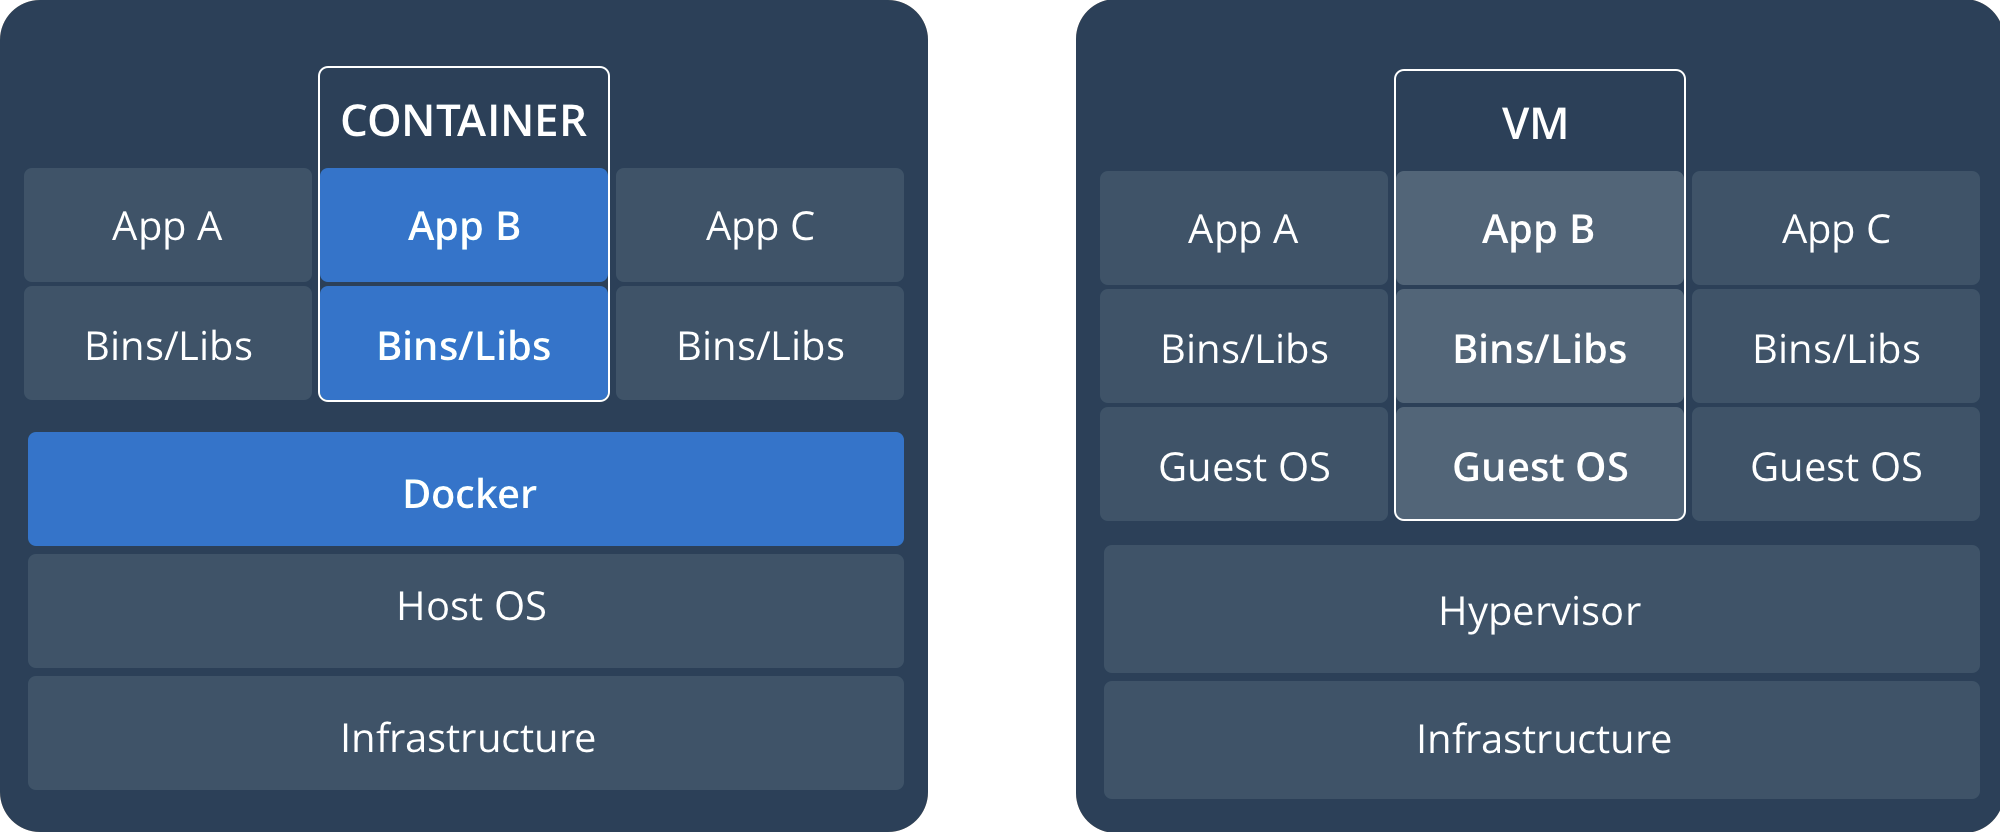
\includegraphics[width=4in]{figures/docker-vs-vm.png}
    \caption[Docker VS VM]
    {Docker VS VM \cite{what_container}}
    \label{fig:DOCKER_VS_VM}
\end{figure}

Die Open Source Plattform Docker ist neben vielen anderen Lösungen einer der bekanntesten Vertreter der Containervirtualisierung und ist Gründer der Open Container Initiative \cite{about_docker}. Erstmals wurde Docker von seinem Erfinder Solomon Hykes im Jahr 2013 der Öffentlichkeit vorgestellt und hat inzwischen die Art und Weise, wie Anwendungen besonders bei Firmen mit vielen Hosts betrieben werden, revolutioniert \cite{docker_adoption}. Durch einen modularen Aufbau und einer Kooperation mit Microsoft unterstützt Docker neben einer Variante mit einer Linux \ac{vm} inzwischen eine native Containervirtualisierung auf Windows \cite{docker_for_windows}. Über den kostenlosen Docker Compose Client lassen sich mehrere unterschiedliche Container zu einem Bundle zusammenfassen \cite{docker_compose} und ermöglichen somit komplexe Anwendungen mit verschiedene Dienste, die jeweils ihren eigenen Ausführungsumgebungen haben. Die verschiedenen Dienste können dabei über das Netzwerk isoliert vom Hostsystem miteinander kommunizieren. Dabei muss diese Kommunikation zwischen den Containern so wie die externe Kommunikation jeweils einzeln freigegeben werden und verfolgt somit das Prinzip Secure-by-Default. Docker ist jedoch nicht bei einer reinen Containervirtualisierung geblieben. Mit der kostenlosen Erweiterung Docker Swarm können mehrere Docker Hosts zu einem einzigen virtuellen Host vereint werden und stellt somit ein Cluster an Docker Hosts zur Verfügung \cite{docker_swarm}. Dabei wird per Default die Kommunikation zwischen den Docker Hosts mit TLS verschlüsselt. Für einen Docker Client ist es dabei unerheblich, ob nun Docker auf demselben Host oder in einem Cluster läuft. Die API bleibt in beiden Szenarien dieselbe und führt zu einem leichten Einstieg mit Docker Swarm.
